\documentclass[12pt]{article}
\usepackage{graphicx}
\usepackage{amsmath}
\usepackage{listings}
\usepackage{xcolor}
\usepackage{hyperref}
\usepackage{geometry}
\geometry{margin=1in}
\usepackage{fancyhdr}
\pagestyle{fancy}
\fancyhf{}
\rhead{Scientific Calculator}
\lhead{Your Name}

\definecolor{codegray}{gray}{0.95}
\lstset{
    backgroundcolor=\color{codegray},
    basicstyle=\ttfamily\small,
    frame=single,
    breaklines=true,
    postbreak=\mbox{\textcolor{red}{$\hookrightarrow$}\space},
    numbers=left,
    numberstyle=\tiny,
    keywordstyle=\color{blue},
    commentstyle=\color{gray},
    stringstyle=\color{orange}
}

\title{Scientific Calculator Using Arduino Uno}
\author{Your Name}
\date{\today}

\begin{document}

\maketitle

\begin{figure}[h]
    \centering
    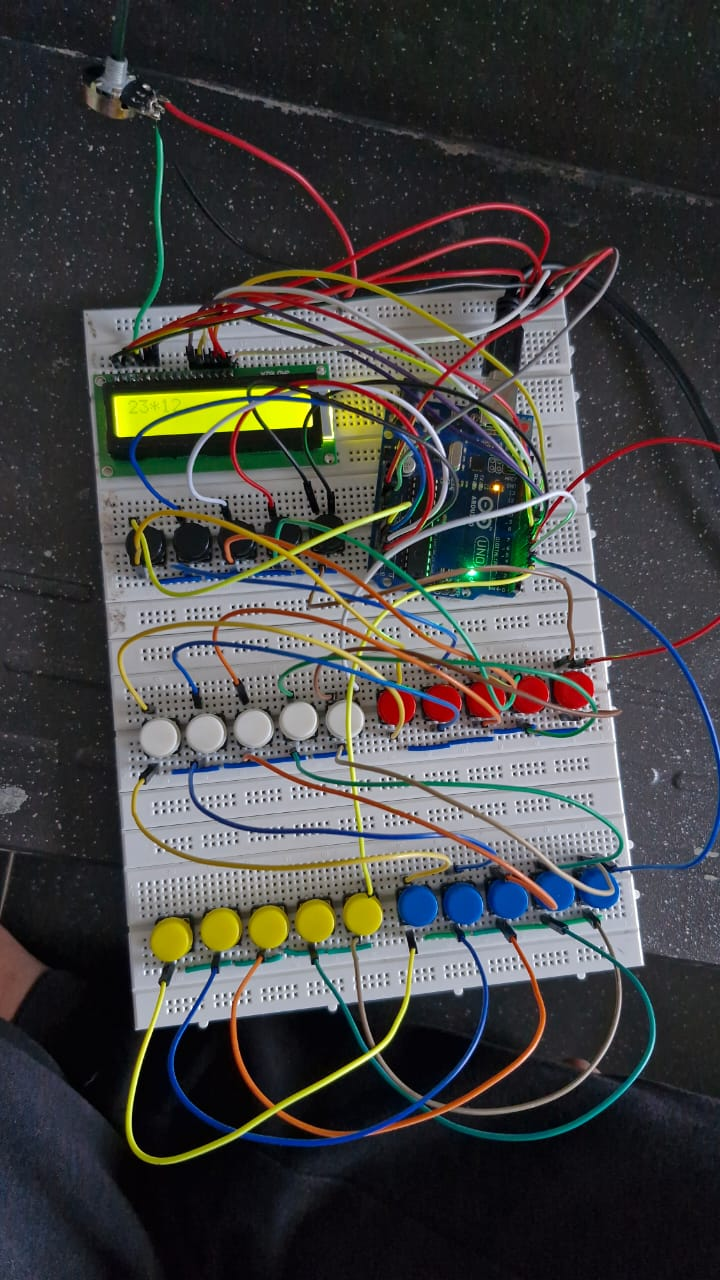
\includegraphics[width=0.6\textwidth]{figs/calculator.jpeg}
    \caption{Scientific Calculator using Arduino}
\end{figure}

\section*{Abstract}
This project demonstrates the implementation of a scientific calculator using an Arduino Uno, a 16x2 LCD, and a 5x5 button matrix. The device evaluates complex mathematical expressions, including nested functions and operations with full BODMAS precedence, using custom numerical methods and parsing techniques.

\section*{Hardware Description}
\begin{itemize}
    \item \textbf{Microcontroller:} Arduino Uno R3
    \item \textbf{Display:} 16x2 LCD (JHD162A) connected to pins 7 to 12
    \item \textbf{Input:} 5x5 matrix keypad using tactile switches
    \item \textbf{Pins Used:}
    \begin{itemize}
        \item Rows: Digital Pins 2 to 6
        \item Columns: Analog Pins A0 to A4
        \item LCD: Pins 7 (RS), 8 (EN), 9-12 (D4-D7)
    \end{itemize}
    \item \textbf{Power:} USB or external adapter via Arduino
\end{itemize}

\section*{Software Overview}
The calculator firmware is written in Arduino C++ using the \texttt{LiquidCrystal} library for display and custom logic for expression parsing. The code includes:

\begin{itemize}
    \item Button matrix scanning
    \item LCD display handling
    \item Recursive expression parser with BODMAS logic
    \item Numerical implementations of sin, cos, log, sqrt, cbrt
\end{itemize}

\section*{Code Explanation}

\subsection*{1. Library and LCD Setup}
\begin{lstlisting}
#include <LiquidCrystal.h>
LiquidCrystal lcd(7, 8, 9, 10, 11, 12);
\end{lstlisting}
This includes the LiquidCrystal library and defines the LCD pins connected to Arduino.

\subsection*{2. Keypad and Mapping}
\begin{lstlisting}
const int rowPins[5] = {2, 3, 4, 5, 6};
const int colPins[5] = {A0, A1, A2, A3, A4};
const char buttonMap[5][5] = {
    {'0', '1', '2', '3', '4'},
    {'5', '6', '7', '8', '9'},
    {'+', '-', '*', '/', '='},
    {'s', 'c', 'l', 'q', 'r'},
    {'(', ')', '.', 'p', 'C'}
};
\end{lstlisting}
Each button in the 5x5 matrix is mapped to a character (digits, operators, functions, etc).

\subsection*{3. Initialization}
\begin{lstlisting}
void setup() {
    lcd.begin(16, 2);
    lcd.print("Sci Calculator");
    delay(1500);
    lcd.clear();
    for (int i = 0; i < 5; i++) {
        pinMode(rowPins[i], OUTPUT);
        digitalWrite(rowPins[i], HIGH);
    }
    for (int j = 0; j < 5; j++) {
        pinMode(colPins[j], INPUT_PULLUP);
    }
}
\end{lstlisting}
Initializes the LCD and sets up the keypad: rows as outputs, columns with pull-ups.

\subsection*{4. Main Loop and Key Scan}
\begin{lstlisting}
void loop() {
    char key = scanKeypad();
    if (key != '\0') {
        handleKeyPress(key);
    }
}
\end{lstlisting}

\begin{lstlisting}
char scanKeypad() {
    for (int i = 0; i < 5; i++) {
        digitalWrite(rowPins[i], LOW);
        for (int j = 0; j < 5; j++) {
            if (digitalRead(colPins[j]) == LOW) {
                delay(200);
                while (digitalRead(colPins[j]) == LOW);
                digitalWrite(rowPins[i], HIGH);
                return buttonMap[i][j];
            }
        }
        digitalWrite(rowPins[i], HIGH);
    }
    return '\0';
}
\end{lstlisting}
Scans each row by pulling it low, reads the columns to detect which button is pressed.

\subsection*{5. Handling Key Press}
\begin{lstlisting}
void handleKeyPress(char key) {
    if (key == 'C') {
        inputExpression = "";
        lcd.clear();
    } else if (key == '=') {
        float result = evaluateExpression(inputExpression);
        lcd.clear();
        if (result == -9999) lcd.print("Error");
        else lcd.print(result);
        inputExpression = "";
    } else if (key == 'p') {
        inputExpression += "3.14159";
        lcd.print("3.14159");
    } else {
        inputExpression += key;
        lcd.print(key);
    }
}
\end{lstlisting}
Handles building the expression string, clearing it, evaluating it, or inserting \(\pi\).

\subsection*{6. Expression Evaluation}
\begin{lstlisting}
float evaluateExpression(String expr) {
    for (int i = 0; i < expr.length(); i++) {
        if (expr[i] == 's' || expr[i] == 'c' || ...) {
            int startIndex = i + 1;
            if (expr[startIndex] != '(') return -9999;
            int endIndex = findMatchingClosingParenthesis(expr, startIndex);
            ...
            float argument = evaluateExpression(argumentStr);
            float computedValue = computeFunction(expr[i], argument);
            expr = expr.substring(0, i) + String(computedValue) + expr.substring(endIndex + 1);
            i = -1;
        }
    }
    return parseBODMAS(expr);
}
\end{lstlisting}
Handles recursive parsing for nested functions like \texttt{sin(log(90))}.

\subsection*{7. Compute Math Functions}
\begin{lstlisting}
float computeFunction(char func, float value) {
    switch (func) {
        case 's': return numericalSin(...);
        case 'c': return numericalCos(...);
        case 'l': return numericalLog(value);
        case 'q': return numericalSqrt(value);
        case 'r': return numericalCubeRoot(value);
        default: return -9999;
    }
}
\end{lstlisting}

\subsection*{8. Parsing BODMAS}
\begin{lstlisting}
float parseBODMAS(String expr) {
    int startParen = expr.indexOf('(');
    while (startParen != -1) {
        int endParen = findMatchingClosingParenthesis(expr, startParen);
        String subExpr = expr.substring(startParen+1, endParen);
        float subResult = parseBODMAS(subExpr);
        expr = expr.substring(0, startParen) + String(subResult) + expr.substring(endParen+1);
        startParen = expr.indexOf('(');
    }
    return evaluateBasicBODMAS(expr);
}
\end{lstlisting}
Recursively evaluates expressions inside parentheses before computing the final result.

\subsection*{9. Operator Precedence Evaluation}
\begin{lstlisting}
float evaluateBasicBODMAS(String expr) {
    // +, -, *, / handled with correct order
    ...
}
\end{lstlisting}
Implements a simplified operator precedence evaluator without using stacks.

\subsection*{10. Numerical Math Implementations}
\begin{lstlisting}
float numericalSin(float x) { ... }
float numericalCos(float x) { ... }
float numericalLog(float x) { ... }
float numericalSqrt(float x) { ... }
float numericalCubeRoot(float x) { ... }
\end{lstlisting}
All functions are implemented using numerical methods like integration or Newton-Raphson.

\section*{Conclusion}
This calculator is capable of evaluating highly complex expressions, supports function nesting, and mimics real scientific calculator behavior. With plans to port this to AVR-GCC, it also serves as a strong embedded systems and parsing logic demonstration.

\section*{Links}
\begin{itemize}
	\item GitHub: \url{https://github.com/mr21sk/my-projects/tree/main/Scientific-Calculator}
\end{itemize}

\end{document}

